\chapter{Výsledková část}
Následující kapitola shrnuje výsledky CFD simulace popsané v předcházejících odstavcích. Na obr. \ref{fig:vecfield} je znázorněno vektorové pole rychlosti kapaliny v řezu nádobou a čase \SI{6}{\second}, což již lze považovat za poměrně ustálený stav. Z obrázku je dobře patrný vznikl sekundárních cirkulačních smyček v prostoru pod míchadlem. Tento jev byl experimentálně pozorován řadou (např. XX) při zvolené světlé výšce míchadla $C=T/3$.  

\begin{figure}[h!]
\begin{center}
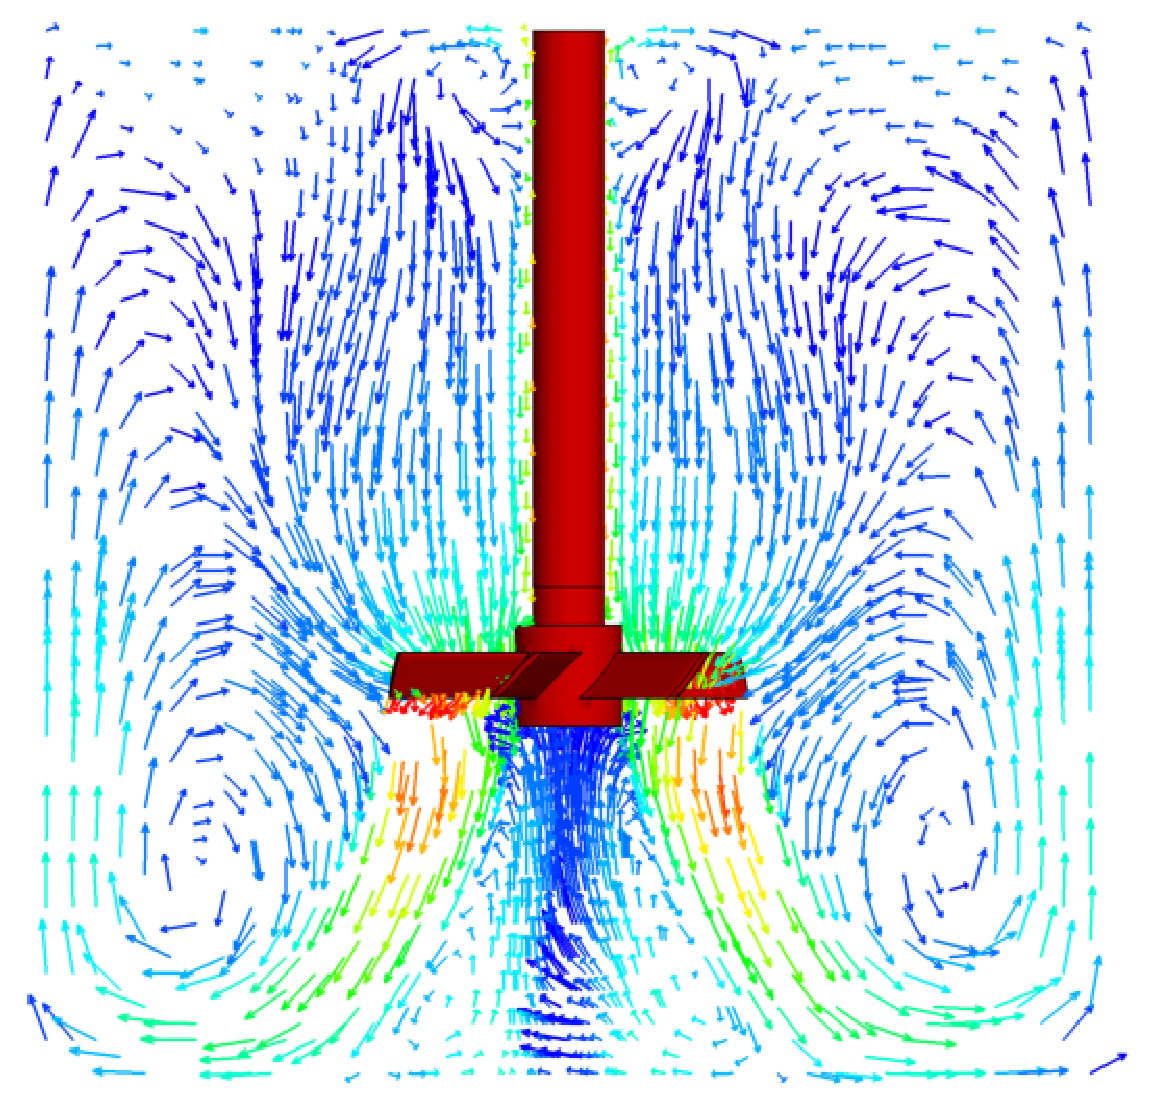
\includegraphics[scale=0.5]{images/vecfield.eps}
\caption{Vektorové pole rychlosti}
\label{fig:vecfield}
\end{center}
\end{figure} 


\begin{figure}[h!]
  \begin{center}
  \subfloat[A gull]{\label{fig:gull}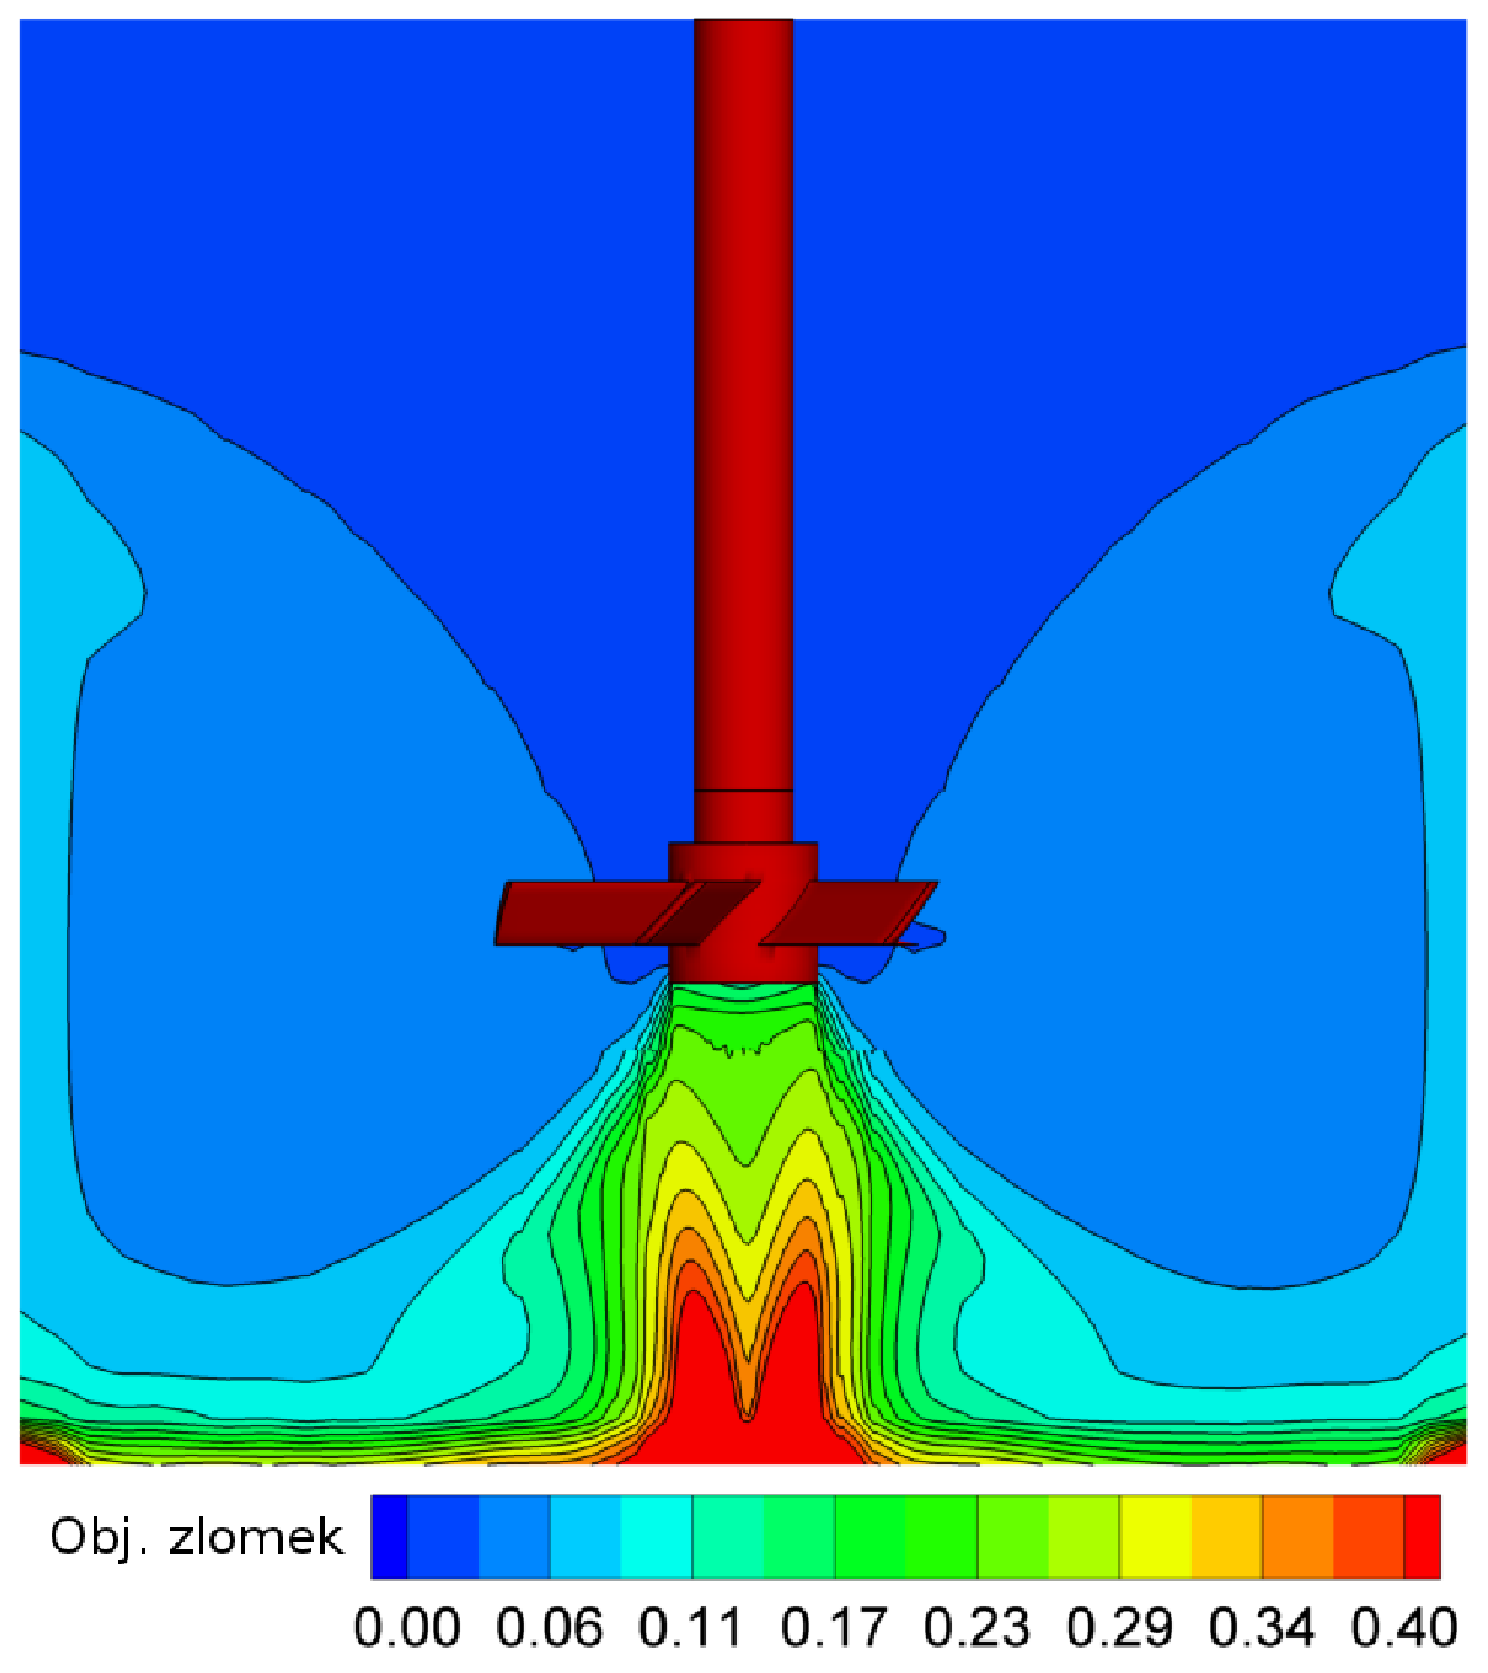
\includegraphics[scale=0.3]{images/volSch-2.eps}}  
  \qquad             
  \subfloat[A tiger]{\label{fig:tiger}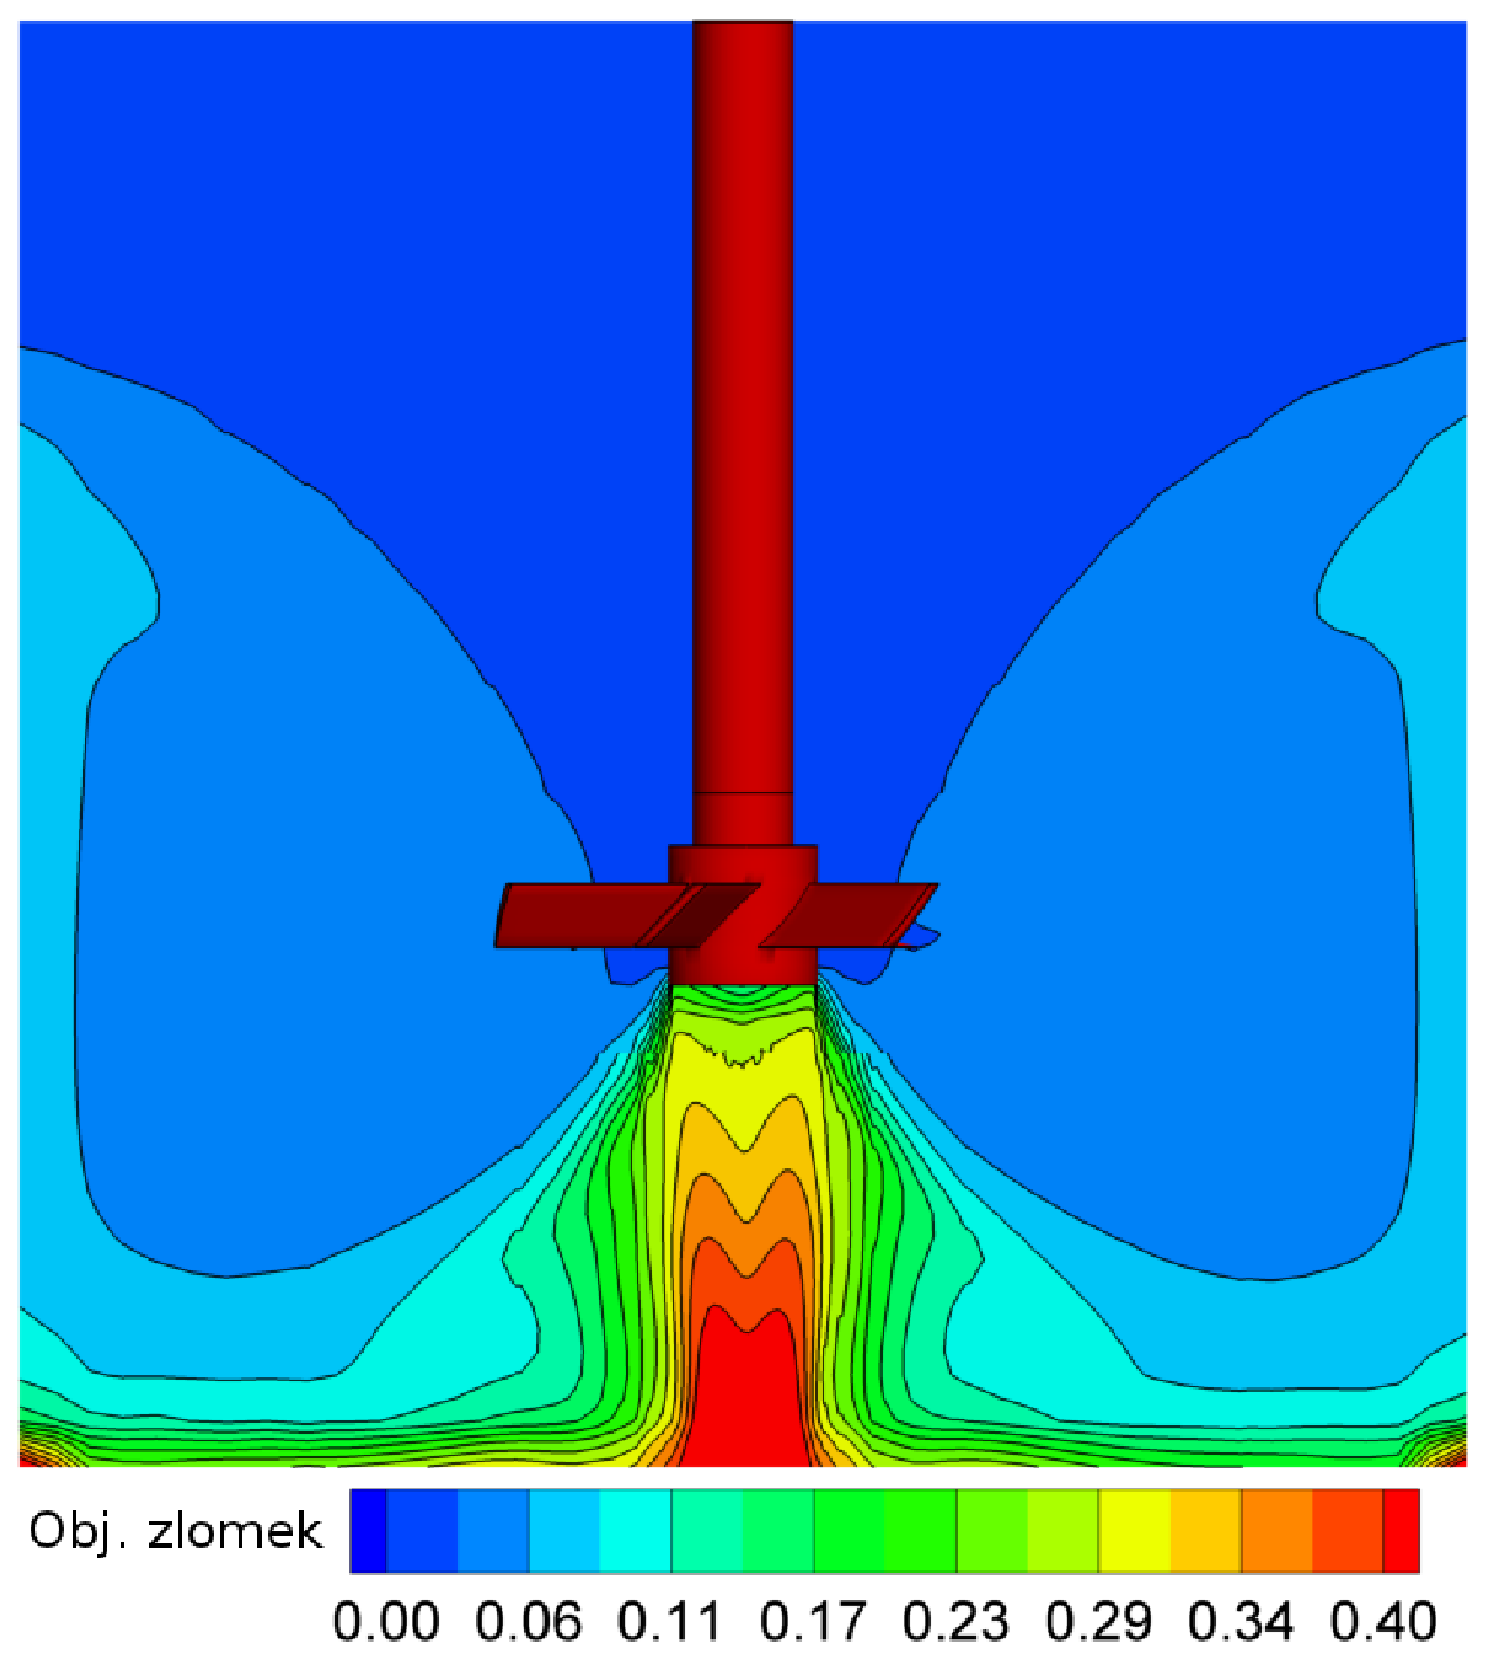
\includegraphics[scale=0.3]{images/volPin-2.eps}}
  \\
  \subfloat[A mouse]{\label{fig:mouse}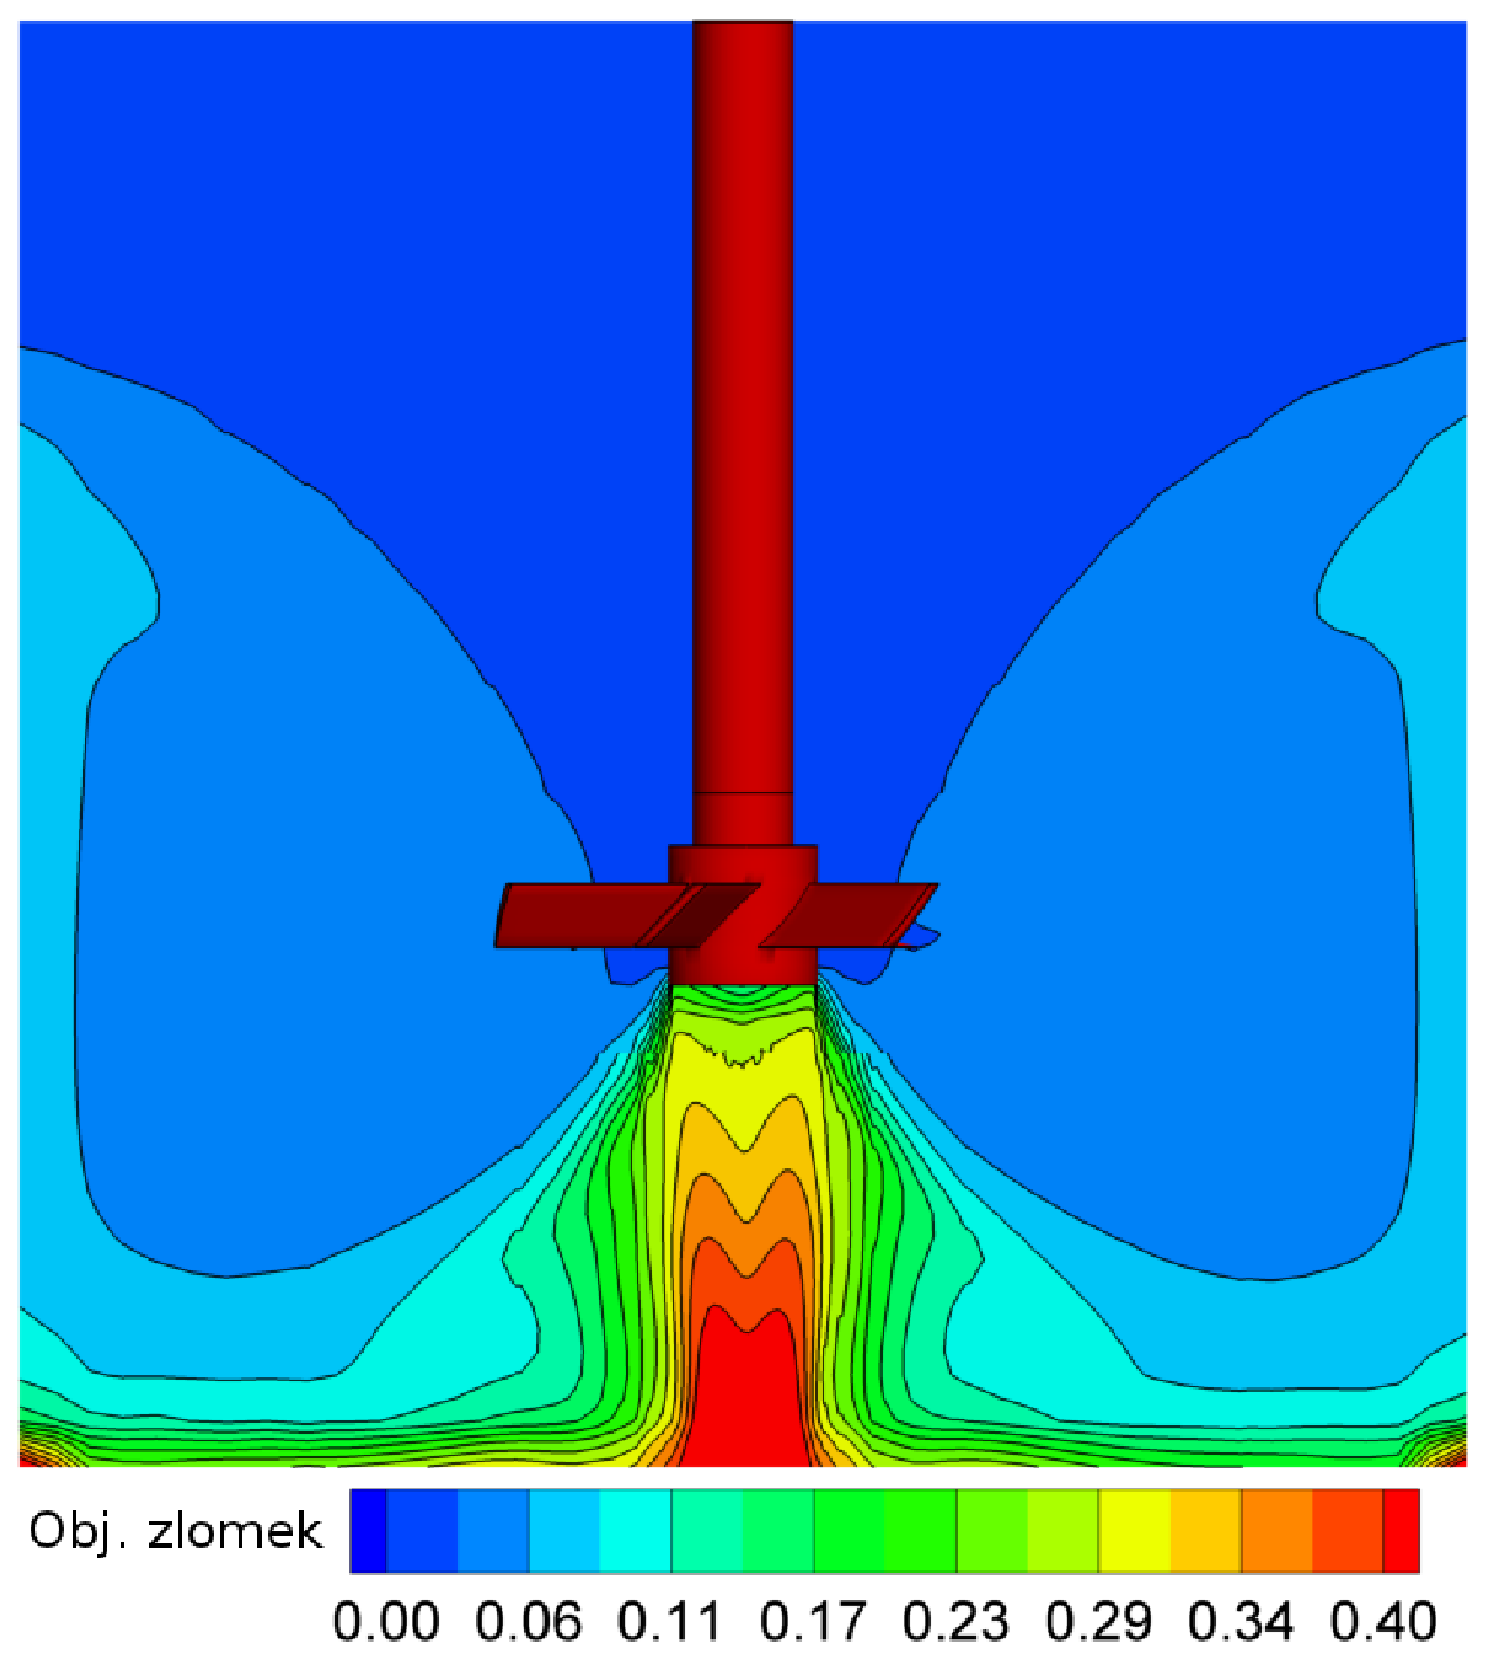
\includegraphics[scale=0.3]{images/volPin-2.eps}}
  \qquad
  \subfloat[A mouse]{\label{fig:mouse}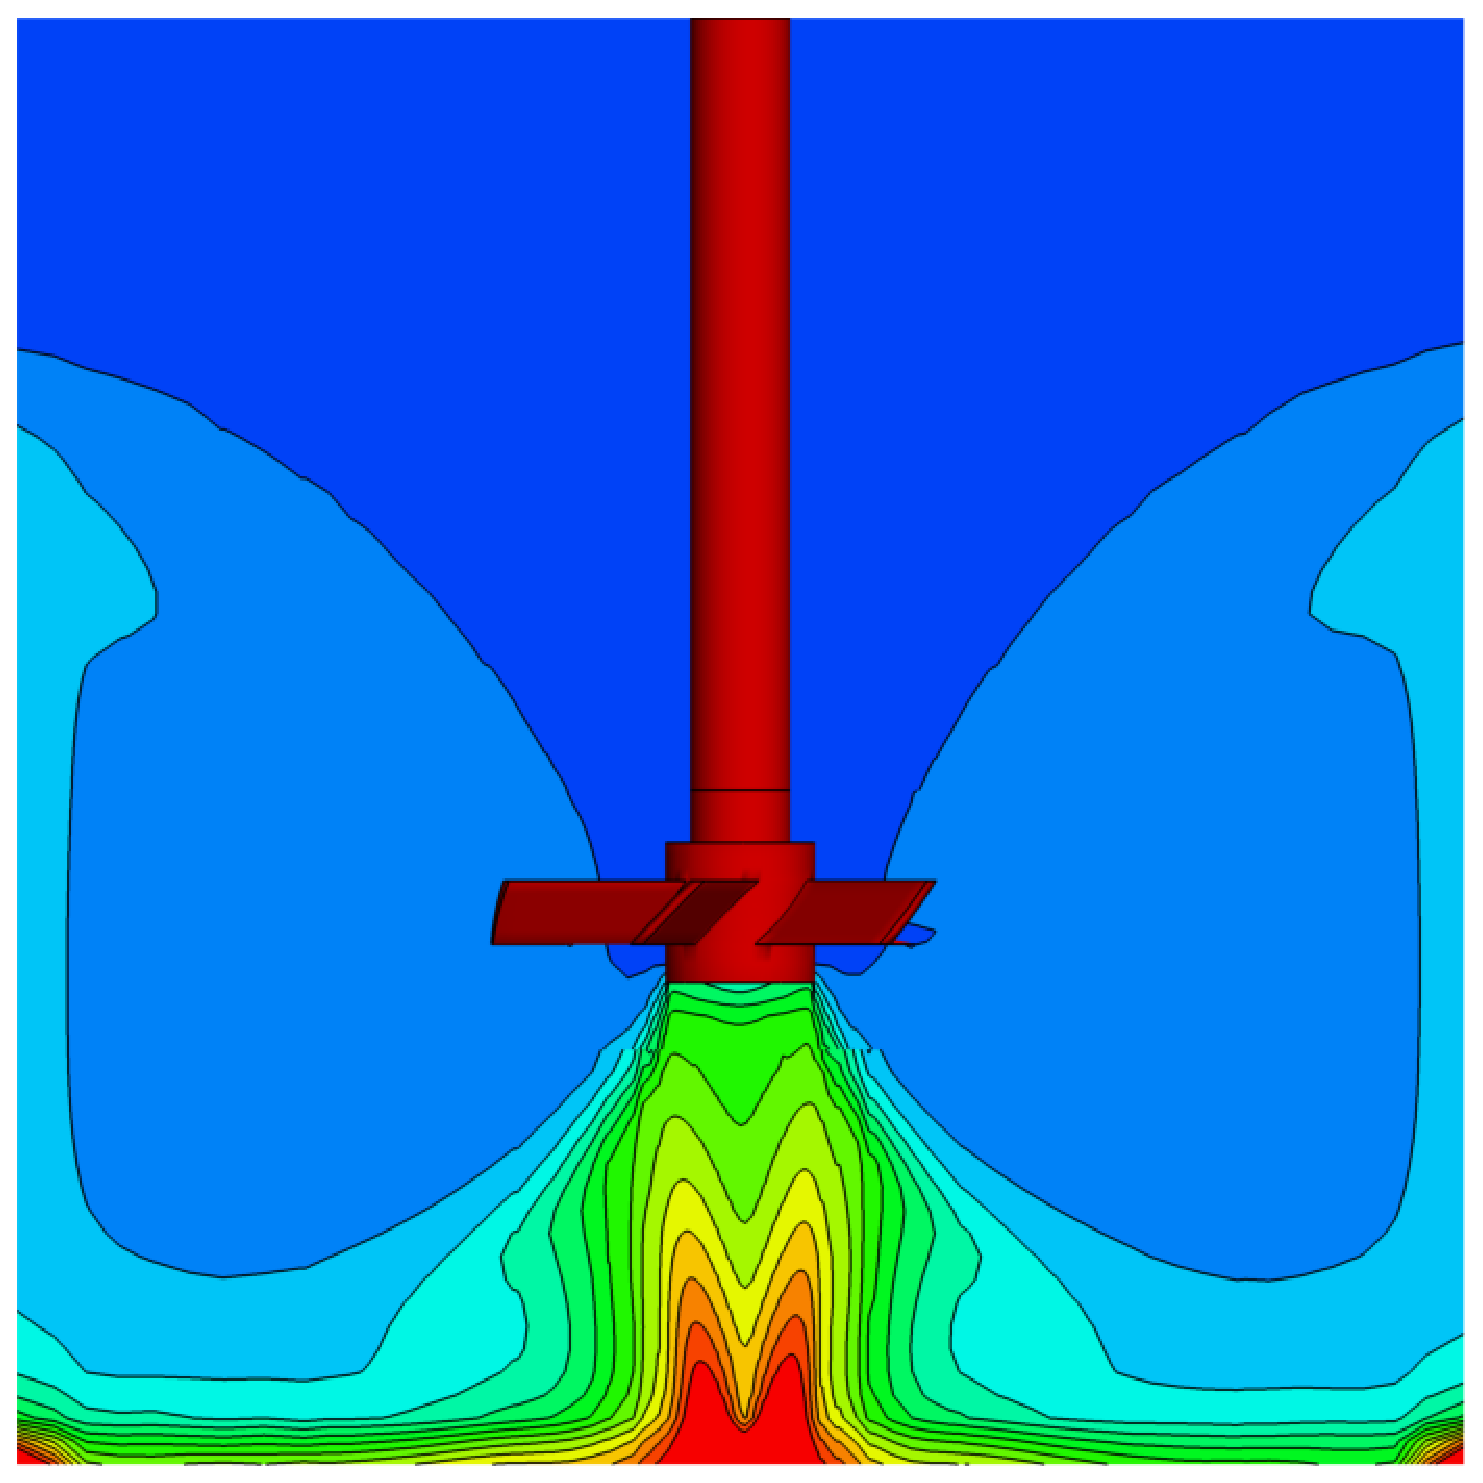
\includegraphics[scale=0.3]{images/volKho-2.eps}}
  \caption{Pictures of animals}
  \label{fig:animals}
  \end{center}
\end{figure}